\documentclass[10pt,twocolumn]{article}

%%% PACKAGE SETTINGS %%%
%% Font settings %%
\usepackage[T1]{fontenc}
\usepackage{charter}
%% Custom title page %%
\usepackage[center,small,sc]{titlesec}
\titleformat{\section}{\normalfont\fontsize{13}{13}\bfseries}{\thesection}{.75em}{}
\titleformat{\subsection}{\normalfont\fontsize{12}{12}\bfseries}{\thesubsection}{.5em}{}

%% Custom margins %%
\usepackage[nohead, nomarginpar, margin=.6in, foot=.35in]{geometry}
\setlength{\columnsep}{2em} % set space between two-column format
\setlength{\parskip}{.25em}

%% BibTeX citation pkg
\usepackage{cite}

%% Footnotes

%% Figures, listings with caption %%
\usepackage{hyperref}
\hypersetup{
  colorlinks,
  linkcolor={red!50!black},
  citecolor={blue!50!black},
  urlcolor={blue!80!black}
}
\usepackage{float}
\usepackage{graphicx}
\usepackage[font=normal,labelfont={bf,it},textfont={bf,it}]{caption}

\usepackage{lipsum}
\usepackage{xcolor}
\usepackage{textcomp}
\usepackage{listings}

\lstset{
  basicstyle=\small\ttfamily,
  commentstyle=\ttfamily,
  keywordstyle=\bfseries,
  aboveskip=1pt,
  belowskip=1pt,
  frame=single,
  captionpos=b,
  showstringspaces=false,
  columns=flexible,
  linewidth=\columnwidth,
  breaklines=true,
  keepspaces=true,
  identifierstyle=\ttfamily,
  keywordstyle=\ttfamily\color[rgb]{0,0,1},
  commentstyle=\ttfamily\color[rgb]{0.133,0.545,0.133},
  stringstyle=\ttfamily\color[rgb]{0.627,0.126,0.941},
}

%%% DOCUMENT BEGINS %%%
\begin{document}
\author{
        Julien Couvy\\
        Vrije Universiteit Amsterdam\\
        \texttt{julien.couvy@gmail.com}
        \and
        Herbert Bos\\
        Vrije Universiteit Amsterdam\\
        \texttt{herbertb@cs.vu.nl}
        \and
        Cristiano Giuffrida\\
        Vrije Universiteit Amsterdam\\
        \texttt{giuffrida@cs.vu.nl}
}
\title{\Huge Mov2Rop: <Find a title :(>\vspace{.75em}}
\maketitle

\begin{abstract}

  \textbf{We present a proof of concept pseudo-compiler that translates a given
    exploit in any language to a return oriented programming payload for a
    target binary. In contrast to other works, we take advantage of the Turing
    completeness of the x86 mov instruction. By only having to handle mov
    instructions instead of the entire ISA, we reduce the complexity of crafting
  payloads while keeping, in theory, the same degree of expresiveness.}

  \textbf{We describe the fundamentals behind ROP attacks, and explain the
    functionning of our tool. In addition, we discuss its limitations and the
    results found using  sample test programs. Finally, we suggest ways to extend
  our work.}

\end{abstract}

\section{INTRODUCTION}

The widespread adoption of \textit{Data Execution Prevention (DEP)}, which
ensures that writable memory regions are non-executable by marking them with a
special flag, such that an attempt to execute machine code in these regions
will cause an exception has largely mitigated classic code injections attacks.
W$\oplus$X was the industry response to code injection exploits, it is deployed
in virtually all main operating systems: Linux (via PaX patches), OpenBSD,
Windows (since XP SP2), OS X (since 10.5), Android and so on\ldots Hardware
constructors also provided easy support with an extra flag dedicated to the
marking: Intel "XD" and AMD "WX" to name a few.

DEP techniques and W$\oplus$X largely killed classic code injection attacks.
However, as one exploit faded another arose. In 1997, Solar Designer presented
a new approach \textit{return-to-libraries}\cite{solar_returnintolib_1997}
attacks. Once the control flow of a program was comprised, the attacker would
use code (functions) already present in shared libraries. No code injection
were required, thus bypassing the defenses we highlighted. A classic target was
\textit{libc}\footnote{return-to-lib attacks are often refered as
return-to-libc for that reason} that contained subroutines for powerful
system calls that would insure arbitrary code execution. Back then, a
common perception was that removing dangerous
\textit{syscalls}\footnote{system() allows to execute any program with the
current \textit{privileges}} would suffice to stop return-to-libc attacks.
Besides, with the avenue of Intel's new 64bits x86 processors, the
subroutines calling convention was changed to require the first argument of
a function to be passed in a register instead of on the stack. Shared
libraries developpers also began to restrict or remove library functions
that performed useful actions for attackers. As a result,
return-to-libraries attacks were much harder to craft successfully and
faded away for a time.

At Black Hat USA 08, Roemer et al.\  presented a Turing-complete exploit
language capable of arbitrary code execution without relying on shared
libraries. \textit{Return Oriented Programming
(ROP)}\cite{roemer_return-oriented_2012} has now become the main technique of
choice for nearly all modern exploits of memory-safety vulnerabilites.

In this paper, we present \textit{Mov2Rop} an attempt at creating a ROP
pseudo-compiler that translates an exploit of choice into a gadget chain for a
target binary. In its current state, the only supported architecture is Intel
x86. One of our motivations was to make use of Domas' single instruction
compiler \textit{movfuscator}\cite{domas_movfuscator} based on the observation
that mov instructions are Turing complete\cite{dolan_mov_2013}. Using
movfuscator, we only have to find gadget chains for mov instructions greatly
reducing the complexity of our tool while keeping, in theory, the ability to
compile any exploit in to its ROP equivalent.


\section{BACKGROUND}

\subsection{Process Memory Organization} 
We will briefly describe the
organization of processes in memory (see \autoref{fig_memorg}) and recap what is the stack. 

Processes are divided into three regions or segments: \textit{Text, Data} and
\textit{Stack}.

\begin{figure}[h]
  \centering
  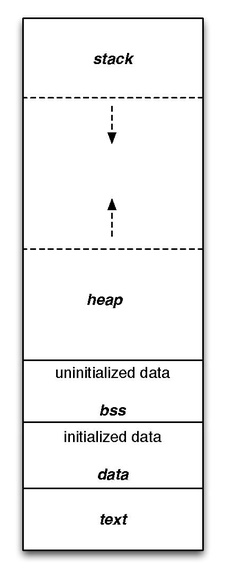
\includegraphics[scale=.85]{./graphics/memory_organization.jpg}
  \caption{Memory organization}
  \label{fig_memorg}
\end{figure}

\textbf{\textit{Text segment:}} also known as code segment, it is fixed by the program, it
includes the executable instructions and read-only data. This region
corresponds to the text section of the executable file. It is normally
marked read-only and any attempt to write to it will result in a segmentation
violation.

\textbf{\textit{Data segment:}} it is split in two part
\begin{itemize}
\item Initializated data, simply called data segment
\item Uninitialized data, also known as the bss segment
\end{itemize}
    The data segment contains the global variables and static variables
which have a pre-defined value and can be modified. The BSS segment contains
all global variables and static variables that are initialized to zero or do
not have explicit initialization in source code.

\begin{lstlisting}[aboveskip=\bigskipamount,belowskip=\medskipamount,caption=Variable
location in memory,language=C] 
// this static variable is stored in the BSS segment
static int bss_variable;
// this global variable is in the DATA segment
int data_variable = 42; 
\end{lstlisting}

\textbf{\textit{Heap segment:}} it is the region where dynamic memory
allocation takes place. The heap area commonly begins at the end of the
\texttt{.bss} and \texttt{.data} segments and grows to larger addresses from
there.

\textit{\textbf{Stack segment:}} a stack is a contiguous block of memory
containing data. It is a \textit{Last In First Out} data structure, which means
literally that the latest value stored on the stack will be the first to be
removed, commonly used
in computers. A register called the \textit{stack pointer} points to
the top of the stack. In addition to the stack pointer, a frame or local base
pointer is also present which points to a fixed location within a frame. Its
size is dynamically adjusted by the kernel at run time.

Every processor \textit{Instruction Set Architecture (ISA)} integrates
instructions to \texttt{push} and \texttt{pop} values onto/off the stack. The stack consists of
logical stack frames that are pushed when calling a function and popped when
returning. A stack frame contains the parameters to a function, its local
variables, and the data necessary to recover the previous stack frame,
including the value of the instruction pointer at the time of the function
call. Depending on its implementation the stack will grow up or down. In the
rest of this paper, we will consider that the stack grows downwards to
reproduce the behavior of Intel processors.

\subsection{Buffer Overflows}

Low level languages directly compiled to machine code such as C/C++ offer wide
possibilites of implementation without the cost of speed. However, this level
of freedom over memory management increases the risk of errors from programmers.
Indeed, many powerful instructions can easily be exploited if used improperly.
Numerous attacks aim at diverting the control flow during the execution of a
program. Buffer overflows still plague many programs and are a main research
topic in computer
security\cite{DBLP:journals/iee/MouzaraniSZ16,DBLP:journals/iee/PadmanabhuniT16,DBLP:conf/ant/LeonB16}.

\lstinputlisting[aboveskip=\medskipamount,belowcaptionskip=0pt,float=h,language=C,firstline=5,label=lst_overflow,caption=Buffer
overflow vulnerability]{./snippets/simple_overflow.c}

A \textit{buffer overflow} attack is an anomaly where a
program, while writing data to a buffer, overruns the buffer's boundary and
overwrites adjacent memory locations. In other words, a buffer overflow condition exists when a program attempts to put more data in a buffer than it can
hold or when a program attempts to put data in a memory area past a
buffer. Overflows can be used to modify return address or code pointers in order
to execute a malicious piece of code, sometimes already exisiting within the
program's space or injected by the attacker. In resume, buffer overflows rely
on two principal fators: 

\begin{itemize}
    \item Low level language's liberal approach to memory handling
    \item Exploiting the filesystem permission
\end{itemize}

With cautious manipulations, an attacker could grant himself unrestricted
priviledge to unpriviledged account or user.

\textbf{\textit{Example:}} \textit{stack-based buffer
overflow}\cite{one_stacksmashing_1996}. When invoking or exiting a standard C
function, the procedure prolog or epilog must be called, this involves saving
the previous variables and allocating space for the new variables; and
vice-versa when the function exits. The previous FP is pushed, a new FP is
created and SP operates with respect to its new local variables.

\textbf{\textit{Procedure:}} in the following \autoref{lst_overflow},
the vulnerability comes from a wrong use of \textit{strcpy()}. The target
information are the size of the buffer and the address of
\textit{exec\_shell()}. The
former will help us overflow the buffer without going too far leading to a
segmentation fault while the latter is the address we want to return to. Any disassembler tool like \textit{gdb} can give us the
information we need to perform the overflow and spawn a shell.

\begin{lstlisting}[aboveskip=\bigskipamount,belowskip=\medskipamount,caption=Gdb
output on simple\_overflow.c]
$ gdb -q simple_overflow
(...)
(gdb) disas vuln_func
Dump of assembler code for function vuln_func:
   0x08048524 <+0>:	push   %ebp
   0x08048525 <+1>:	mov    %esp,%ebp
   0x08048527 <+3>:	sub    $0x78,%esp
   0x0804852a <+6>:	sub    $0x8,%esp
   0x0804852d <+9>:	pushl  0x8(%ebp)
   0x08048530 <+12>:	lea    -0x6c(%ebp),%eax
   0x08048533 <+15>:	push   %eax
   0x08048534 <+16>:	call   0x80483a0 <strcpy@plt>
   0x08048539 <+21>:	add    $0x10,%esp
(...)
(gdb) print exec_shell
$1 = (...) 0x80484fb <exec_shell>
\end{lstlisting}

To overwrite the return address with the one of \textit{exec\_shell()} we need
to fill the buffer with $100$ bytes, overwrite SFP\footnote{the saved frame
pointer (old content of \%ebp) is called SFP} with a dummy value and then the
target address.

\begin{lstlisting}[aboveskip=\bigskipamount,belowskip=\medskipamount,caption=Stack before and after overflow]
| <argument>                 |
| <return address>           |
| <old %ebp>                 | <= %ebp
| <0x6c bytes of             |
|       ...                  |
|       buffer>              |
| <argument>                 |
| <address of buffer>        | <= %esp
           BEFORE

| 0x80484fb <exec_shell()>   |
| 0x42424242 <fake old %ebp> | "BBBB" in hex
| 0x41414141 ...             | "AAAA" in hex
|   ... (0x6c bytes of 'A's) |
|   ... 0x41414141           |
           AFTER
\end{lstlisting}

In practice, once the return address is overwritten, the attacker can perform
his exploit via a \textit{code injection} assuming no defenses are in place,
\textit{return-to-libraries} attack, or \textit{return oriented programming}
attack.

\begin{lstlisting}[float=ht,belowskip=\medskipamount]
$ ./simple_overflow "$(python2 -c 'print "A"*0x6c + "BBBB" + "\xfb\x84\x04\x08"')"
Spawning a shell !
sh-4.4$
\end{lstlisting}

\subsection{Return Oriented Programming}
In this section we will introduce the concepts behind \textit{return-oriented programming
}\cite{roemer_return-oriented_2012}.

Return-oriented programming is a technique by which an attacker can induce
arbitrary behavior in a program whose control flow he has diverted, without
injecting any code. It was built to overcome buffer exploit defense
mechanisms like ASLR, DEP or W$\oplus$X. The technique consists of aggregating
malicious computation by linking together short code snippets called
\textit{gadgets}.  A \textit{gadget} ends in a \texttt{ret} instruction and is
located in a subroutine within the program's address space. Chained together,
these gadgets allows an attacker who controls the call stack to build and
execute his payload. Because the executed code is stored in memory marked
executable, the W$\oplus$X defense will not prevent it from running.

ROP can be seen as a generalization of traditional return-into-lib attacks. But
the threat is more general. In theory, ROP can be used to make Turing complete
attacks. However, in practice, it requires a really complex work and very
little research concluded to a satisfying automated method of crafting Turing complete
exploits.

\textbf{\textit{Example:}} see \autoref{lst_ropchain}. We want to give a
general understanding on how gadget chaining generaly works. Here, we need to
concatenate \texttt{"/bin/sh"} in a buffer by chaining functions together and
finally spawn a shell. Each functions requires specific parameters that we need
to store on the stack along with the gadget chain.We supposedly found a memory
vulnerability that allows us to perform a stack-buffer overflow in the same
conditions as the last example.

\textbf{\textit{Stack preparation:}} an attacker prepares a fake stack frame to
look like a collection of new return addresses for control-flow changes. In
practice, it is a very meticulous process as we will see in a following
section.

\textbf{\textit{Procedure:}} when the \textit{instruction pointer} points at
the address of \texttt{add\_bin()}, the return address\footnote{see standard C
 function calling procedure} is the address of a
 \texttt{pop; ret;} gadget. The test value is parsed as argument in
 \texttt{add\_bin()}. The \texttt{pop; ret;} gadget ensures that the next value
 pointed by \texttt{\%ip} will be the address of the second gadget in the
 chain. See Appendix \ref{appendix:a} for a written exploit.

\lstinputlisting[aboveskip=\medskipamount,belowcaptionskip=0pt,float=h,language=C,firstline=31,lastline=53,label=lst_ropchain,caption=ROP
exploit example]{./snippets/chaining_func.c}

\begin{lstlisting}[float,aboveskip=\bigskipamount,belowskip=\medskipamount,caption=Stack
prepared with a ROP chain]
| <address of exec_command()> |
| 0xcafebabe <key1>           |
| 0x8badfood <key2>           |
| <address of POP; POP; RET>  |
| <address of add_sh()>       |
| 0xdeadbeef <key>            | <argument>
| <address of POP; RET>       | <return addr>
| <address of add_bin()>      | <function call>
| 0x42424242 <fake old %ebp>  |
| 0x41414141 ...              |
|   ... (0x6c bytes of 'A's)  |
|   ... 0x41414141            | 0x41414141 == "AAAA"
\end{lstlisting}


\section{RELATED WORK}

\textit{Control flow integrity (CFI)} regroup techniques which prevents malwares
attacks from redirecting the flow of execution of a program. Many techniques
were/are being developped to maintain control-flow integrity. However, recent
research also showed that many of these (dated) defenses can be bypassed.

\textit{Address Space Layout Randomization:} ALSR makes it more difficult for
an attacker to predict target addresse. It rearranges the address space
positions of key data areas of a process, including the base of the executable
and the positions of the stack, heap and libraries.

\textit{ShadowStacks\cite{Sinnadurai_transparentruntime}:} This technique
mitigates return address overwrites by keeping a record of of the legitimate
return address for some function call, and then to check that the return
address is still correct before returning.

\textit{Stack Canaries:} They are used to detect a stack buffer overflow before
execution of malicious code can occur. Stack canaries work by modifying every
function's prologue and epilogue regions to place and check a value on the
stack respectively. As such, if a stack buffer is overwritten during a memory
copy operation, the error is noticed before execution returns from the copy
function.

While these techniques improved our defenses against ROP attacks, most of them only
 complexify the infection vector but do not fix the underlying vulnerability.

\textbf{\textit{ROP Compiler:}} Follner et al.\ presented
PSHAPE\cite{barthe_pshape:_2016}, a state-of-the-art open source gadget
chaining tool adapted to realistic scenarios. It offers syntactic and semantic
gadget search and automatic chaining for 64 bits architectures.  They claim
being the only one amongst competition to successfully create ROP chains
automatically in nine out of eleven practical cases.


\section{MOV2ROP}

In this paper, we are trying to translate a given exploit into a ROP chain for
a target binary. Our work differ from other compilers as we chose to compiled
the source code into mov instructions only using an external compiler
\textit{movfuscator}. Mov2Rop is written in Python and is divided into three
different modules: the \textit{Extractor}, \textit{Dissassembler}, and
\textit{Matcher}.

\subsection{Gadget Extraction}
We use Ropper's engine\cite{sashs_ropper} within the Extractor  module to
extract gadgets from binaries. Gadgets are searched according to a regular
expression.

\begin{lstlisting}[float=h,aboveskip=0pt,belowskip=0pt]
$ ropper --file target_bin --search "pop e??; ret;"
0x080bbf26: pop eax; ret;
0x08048411: pop ebp; ret;
0x080481d1: pop ebx; ret;
...
\end{lstlisting}

The output is then parsed by our program to create a list of \textit{Gadget}
objects. Gadgets are defined by a list of \textit{Instruction} objects and the
address of its first instruction. We define an Instruction by a label, an
address, a mnemonic, a source and a destination (without optional offsets).
Mnemonics are short strings representing the type of instruction. A mnemonic is
assigned by looking-up in a dictionnary of opcodes. The opcode is extracted
with regular expressions manipulations on Ropper's output.


\subsection{Payload Treatment}
\begin{itemize}
    \item introducing Capstone framework
    \item how are instructions "tokenized"
\end{itemize}
\subsection{Instruction Analysis}
\begin{itemize}
    \item What rules are applied to each gadget and why
\end{itemize}
\subsection{Gadget chaining}
\begin{itemize}
    \item How the chaining algorithm works (+ pseudo code or/ flowchart ?)
    \item Example (in appendix?) or explained here
\end{itemize}
\subsection{Limitations}
\begin{itemize}
    \item Description of the tool's limitations, discussion of their impact and
        how/if they should be handled ?
    \item (ex: target architecture, input language, liveness, etc...)
\end{itemize}



  
\section{RESULTS \& CONCLUSION}
  We tested our tool on two sample programs written in C. For each case, the
  target binary is the program compiled with a static version of \textit{glibc}
  (see Appendix \ref{appendix:a}).
  We demonstrated a simple yet powerful way to craft return oriented payloads
  which are still to this day a strong attack vector. By exploiting the Turing
  completeness of mov instructions coupled with a mov-compiler, we greatly
  simplified the work needed to implement the exploits. The potential of ROP
  attacks is mainly hindered by the complexity of crafting gadget chains in real
  life scenarios. However, it is possible to find automated ways to handle this
  work making ROP attacks an even bigger threat.

\section{FURTHER WORK}
\begin{itemize}
    \item How to improve our tool
    \item LLVM migration ?
    \item extending supported instructions
    \item payload generator from the gadget chain
    \item side-effect management
\end{itemize}


\section{REFERENCES}
\begingroup
\renewcommand{\section}[2]{}
\bibliographystyle{ieeetr}
\small\bibliography{references}
\endgroup

\appendix
\clearpage
\section{Appendix}
\label{appendix:a}
\begin{table}[!ht]
  \centering
  \lstinputlisting[caption=Fibonacci.c,language=C]{../test_programs/fibonacci.c}
  \medskip

  \begin{tabular}{l|l|l}
    \textbf{Total Instructions} & \textbf{1270} & \textbf{100\%} \\ \hline
    Supported                   & 1042          & 82\%           \\ \hline
    Supported (w/o offsets)     & 962           & 75\%           \\ \hline
    Not supported               & 228           & 17\%          
  \end{tabular}%
  \label{result-fibo}
  \caption{Statistics on fibonacci.c}

  \bigskip

  \lstinputlisting[caption=Hanoi\_towers.c,language=C]{../test_programs/hanoi_towers.c}
  \medskip

  \begin{tabular}{l|l|l}
    \textbf{Total Instructions} & \textbf{2054} & \textbf{100\%} \\ \hline
    Supported                   & 1071          & 82\%           \\ \hline
    Supported (w/o offsets)     & 1579          & 76\%           \\ \hline
    Not supported               & 353           & 17\%          
  \end{tabular}%
  \label{result-hanoi}
  \caption{Statistics on hanoi\_towers.c}
\end{table}

\lstinputlisting[float,label=lst_ropexploit,caption=ROP exploit in Python,language=Python]{./snippets/rop_chain.py}

\end{document}
